% Provenance (never printed): old terminale S material on the disappearance of
% mountain ranges (erosion, transport, sedimentation, isostatic rebound, the
% recycling of continental material). Owner (Sync 0/1): denudation rate,
% sediment load (bed, suspended, dissolved), isostatic rebound, detrital rock,
% diagenesis. Weathering, erosion, deposition are Book 1's (g5); hydrolysis and
% clay minerals g10.07's; discharge g10.08's; isostasy and Airy's model g11.03's;
% sedimentary basin g11.09's; mountain root g12.01's; metamorphism g12.03's;
% half-life is physics' (recalled in prose). Figures: figdata/grade-12/relief_decay.py
% (rates, decay curves, the Varden unconformity from figdata/shared/region.py).
\chapter{هدم الجبال}\label{ch:g12:destruction-of-mountains}

تبدو جبال الأبالاش في شرق أمريكا الشمالية، كما تُرى من محطة الفضاء الدولية،
نقشًا لافتًا من حواف طويلة داكنة تكسوها الغابات وأودية شاحبة
مزروعة، يمتد منها في الصورة أدناه أكثر من \qty{500}{km}.
فالحواف طبقات صخرية
صلبة طُويت \omterm{def:g12:mountain-building:fold}{طيات} متقاربة حين دفعت إفريقيا أمريكا الشمالية، في العصرين
الكربوني والبرمي، قبل أكثر من 250 مليون سنة. وأعلى قممها اليوم، جبل
ميتشل، وهو أعلى نقطة شرق نهر المسيسيبي، يرتفع
\qty{2037}{m} فوق مستوى سطح البحر، أي أقل من ربع ارتفاع إيفرست.
% ledger: photo:g12-appalachians, usgs:alleghanian, usgs:alleghanian-age, ics:base.Triassic, ncparks:mitchell (6684 ft), tht:everest (Book 1 row, 8848.86 m)

\begin{omfigure}
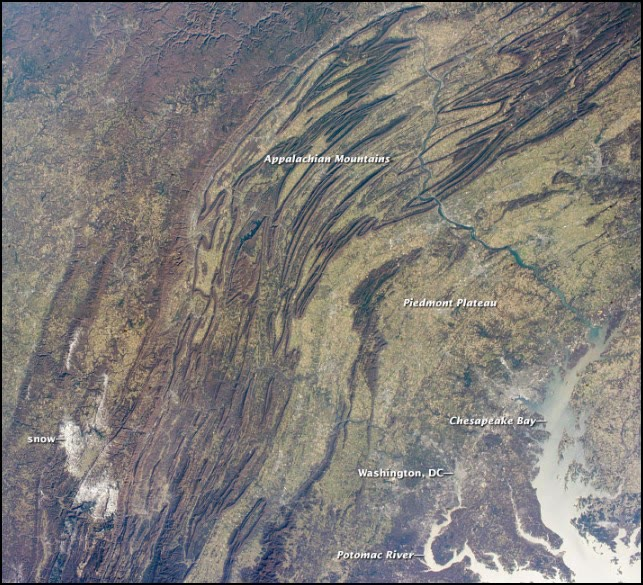
\includegraphics[width=0.6\linewidth]{images/book2/g12-iss-appalachians.jpg}

{\small جبال الأبالاش ذات الأودية والحواف، من شمال شرق بنسلفانيا
(في أعلى اليمين) إلى فرجينيا الغربية، كما صُوّرت من محطة الفضاء
الدولية في 17 نوفمبر 2012. فالحواف المكسوة بالغابات طبقات صخرية صلبة،
والأودية المزروعة طبقات أطرى. الصورة: ناسا (ملك عام).}
\end{omfigure}
% ledger: photo:g12-appalachians

لا تدوم السلسلة الجبلية. فمنذ اللحظة التي ترتفع فيها، يهاجمها المطر والجليد
والأنهار؛ والصخر الذي تحمله ينتهي إلى البحر، فيصير هناك صخرًا
جديدًا. يقيس هذا الفصل سرعة ذلك، ويتتبع الحطام
إلى المكان الذي يتحول فيه إلى حجر، ويبيّن لماذا تظل السلسلة التي
تُبرى وتُستهلك ترتفع في أثناء ذلك.

\begin{recall}
التجوية تفتّت الصخر في مكانه؛ والتعرية تنقل الحطام بعيدًا،
والترسيب يضعه في مكان آخر (الكتاب 1، الصف 5). \omterm{def:g10:soil-formation:chemical-weathering}{والتجوية الكيميائية}
تحوّل الفلسبارات إلى \omterm{def:g10:soil-formation:clay}{معادن طينية} \omterm{def:g10:soil-formation:hydrolysis}{بالحلمهة}
(\cref{ch:g10:soil-formation}). \omterm{def:g10:drainage-basins:discharge}{وتصريف} النهر هو حجم
الماء الذي يمر بنقطة في الثانية (\cref{ch:g10:drainage-basins}). وتطفو
القشرة على الوشاح في \omterm{def:g11:lithosphere-asthenosphere:isostasy}{توازن أيزوستاتي}؛ وفي نموذج إيري، المنطقة التي قشرتها
أسمك بمقدار $\Delta H$ ترتفع أعلى بمقدار $\Delta H\,(\rho_m - \rho_c)/\rho_m$
(\cref{ch:g11:lithosphere-asthenosphere})، والسلسلة العالية ترتكز على \omterm{def:g12:continental-crust:root}{جذر}
من قشرة سميكة (\cref{ch:g12:continental-crust}). وتتراكم الرسوبيات في
\omterm{def:g11:fossil-fuel-geology:basin}{الأحواض الرسوبية} (\cref{ch:g11:fossil-fuel-geology}). والصخور المدفونة عميقًا في
حزام جبلي تتحول (\cref{ch:g12:metamorphic-rocks}).
\end{recall}

\section{ما سرعة بري اليابسة؟}

\begin{definition}[معدل التجريد]\label{def:g12:destruction-of-mountains:denudation}
\emph{معدل التجريد}\index{معدل التجريد} لمنطقة ما هو متوسط
سمك الصخر الذي تزيله منها التجوية والتعرية معًا في
وحدة الزمن. ويُعطى عادة بالأمتار في كل مليون سنة
(\unit{m/Myr})، وهو يساوي الملّيمترات في كل ألف سنة.
\end{definition}
% ledger: pb11:rates (rates in m/Myr), earle:loads

كيف يُقاس شيء بهذا البطء؟ تصطدم الأشعة الكونية بالأرض فتصنع
نظيرًا نادرًا، البيريليوم-10، في كوارتز الأمتار القليلة العليا من الصخر.
وكلما كان بري السطح أبطأ، طال بقاء كل حبيبة قرب الأعلى،
وزاد ما تجمعه من البيريليوم-10. وقياسه في رمل نهر
يعطي متوسط \omterm{def:g12:destruction-of-mountains:denudation}{معدل التجريد} للحوض كله عند المنبع، على مدى
آلاف إلى ملايين من السنين الماضية.
% ledger: pb11:rates (10Be produced within a few metres of the surface; concentration reflects near-surface residence time; 10^3 to 10^6 years)

وجدت مجموعة من 1599 قياسًا من هذا النوع أن النتوءات الصخرية العارية
تُبرى ببطء، بمعدل \qty{12}{m/Myr} في المتوسط (والوسيط
\qty{5.4}{m/Myr})، ولا يزيد معدلها قط على \qty{140}{m/Myr}. أما أحواض
\omterm{def:g10:drainage-basins:discharge}{التصريف} كاملة فتفقد أكثر من ذلك بكثير، \qty{218}{m/Myr} في المتوسط، لكن بوسيط
لا يتجاوز \qty{54}{m/Myr}: فقليل من الأحواض السريعة يرفع المتوسط. وأسرعها
أشدها انحدارًا: فمتوسط انحدار الحوض هو العامل الذي يتنبأ أفضل من غيره
بمعدله. والأحواض الواقعة في المناطق النشطة زلزاليًا، حيث ترتفع الجبال،
تتعرى بنحو ضعف سرعة الأحواض الواقعة في المناطق الهادئة.
% ledger: pb11:rates

\begin{omfigure}
\begin{tikzpicture}
\begin{axis}[omrecord, xbar, xmode=log, log origin=infty, bar width=7pt, bar shift=0pt,
  width=0.62\linewidth, height=6.6cm, scale only axis, xmin=3, xmax=1000,
  ymin=0.4, ymax=10.6, ytick={1,...,10}, y tick label style={font=\scriptsize, align=right},
  yticklabels={{النتوءات، الوسيط}, {النتوءات، المتوسط}, {أنهار العالم، بالميزانية}, {الأحواض، الوسيط},
    {المسيسيبي قبل 1900، بالميزانية}, {الأحواض الجافة، المتوسط}, {الأحواض الهادئة، المتوسط}, {الأحواض، المتوسط},
    {الأحواض النشطة زلزاليًا، المتوسط}, {الأحواض القطبية، المتوسط}},
  xlabel={\foreignlanguage{arabic}{معدل التجريد \babelsublr{(\unit{m/Myr})}، بمقياس لوغاريتمي}}, ymajorgrids=false,
  unbounded coords=discard, nodes near coords, nodes near coords align={horizontal}, nodes near coords style={font=\scriptsize},
  point meta=rawx, every node near coord/.append style={/pgf/number format/.cd, fixed, precision=0}]
% computed in figdata/grade-12/relief_decay.py; ledger: pb11:rates, mm10:mississippi, kammerer:mississippi, earle:loads, cm95:crust
\addplot[fill=omThm!45, draw=omThm, every node near coord/.append style={/pgf/number format/.cd, fixed, precision=1}] table[x=measured, y=idx] {figdata/out/grade-12-relief_decay-rates.dat};
\addplot[fill=omDef!45, draw=omDef] table[x=budget, y=idx] {figdata/out/grade-12-relief_decay-rates.dat};
\end{axis}
\end{tikzpicture}

{\small \omterm{def:g12:destruction-of-mountains:denudation}{معدلات تجريد} مقيسة بالبيريليوم-10 (بالأحمر: 1599 قياسًا،
منها 1149 في رمل الأنهار)، ومعدلان حُسبا في هذا الفصل من
الرسوبيات التي تحملها الأنهار (بالأزرق). المصادر: بورتنغا وبيرمان (2011)؛
ميد ومودي (2010)؛ سيفيتسكي وآخرون (2005).}
\end{omfigure}
% values: world_m_per_myr 43.5, miss_before_1900_m_per_myr 55.8 (relief_decay.py)

\section{الأنهار تحمل الجبال بعيدًا}

يغادر كثير مما يُبرى من اليابسة في الأنهار.

\begin{definition}[الحمولة الرسوبية]\label{def:g12:destruction-of-mountains:load}
\emph{الحمولة الرسوبية}\index{حمولة رسوبية} لنهر ما هي المادة التي
يحملها، في ثلاث صور: \emph{الحمولة القاعية}\index{حمولة قاعية}، وهي حبيبات كبيرة
تتدحرج أو تُدفع أو تقفز على طول القاع؛ و\emph{الحمولة
العالقة}\index{حمولة عالقة}، وهي حبيبات صغيرة يحملها الماء المتحرك؛
و\emph{الحمولة الذائبة}\index{حمولة ذائبة}، وهي أيونات في محلول، مثل
الكالسيوم والكلوريد، خلّفتها \omterm{def:g10:soil-formation:chemical-weathering}{التجوية الكيميائية}.
\end{definition}
% ledger: earle:loads

تبلغ \omterm{def:g12:destruction-of-mountains:load}{الحمولة الذائبة} في المتوسط نحو \qty{15}{\percent} من الكتلة التي
يحملها النهر. وكلما كان الماء أسرع، كبرت الحبيبات التي يستطيع رفعها. فحبيبة
رمل قطرها \qty{1}{mm} تُرفع من القاع عند نحو
\qty{20}{cm/s}، وما إن تتحرك حتى تبقى عالقة إلى أن ينخفض التيار
إلى ما دون \qty{10}{cm/s}. وحبيبات الغرين أصعب رفعًا من الرمل،
لأنها يلتصق بعضها ببعض: فحبيبة قطرها \qty{0.01}{mm} تحتاج إلى
\qty{60}{cm/s} لتُرفع، لكن تيارًا سرعته \qty{0.1}{cm/s} يكفي بعد ذلك لإبقائها
عالقة. ولهذا تجري الأنهار في فيضانها بلون بني، ولهذا يقطع أدق الوحل
الطريق كله إلى البحر.
% ledger: earle:loads

\begin{omfigure}
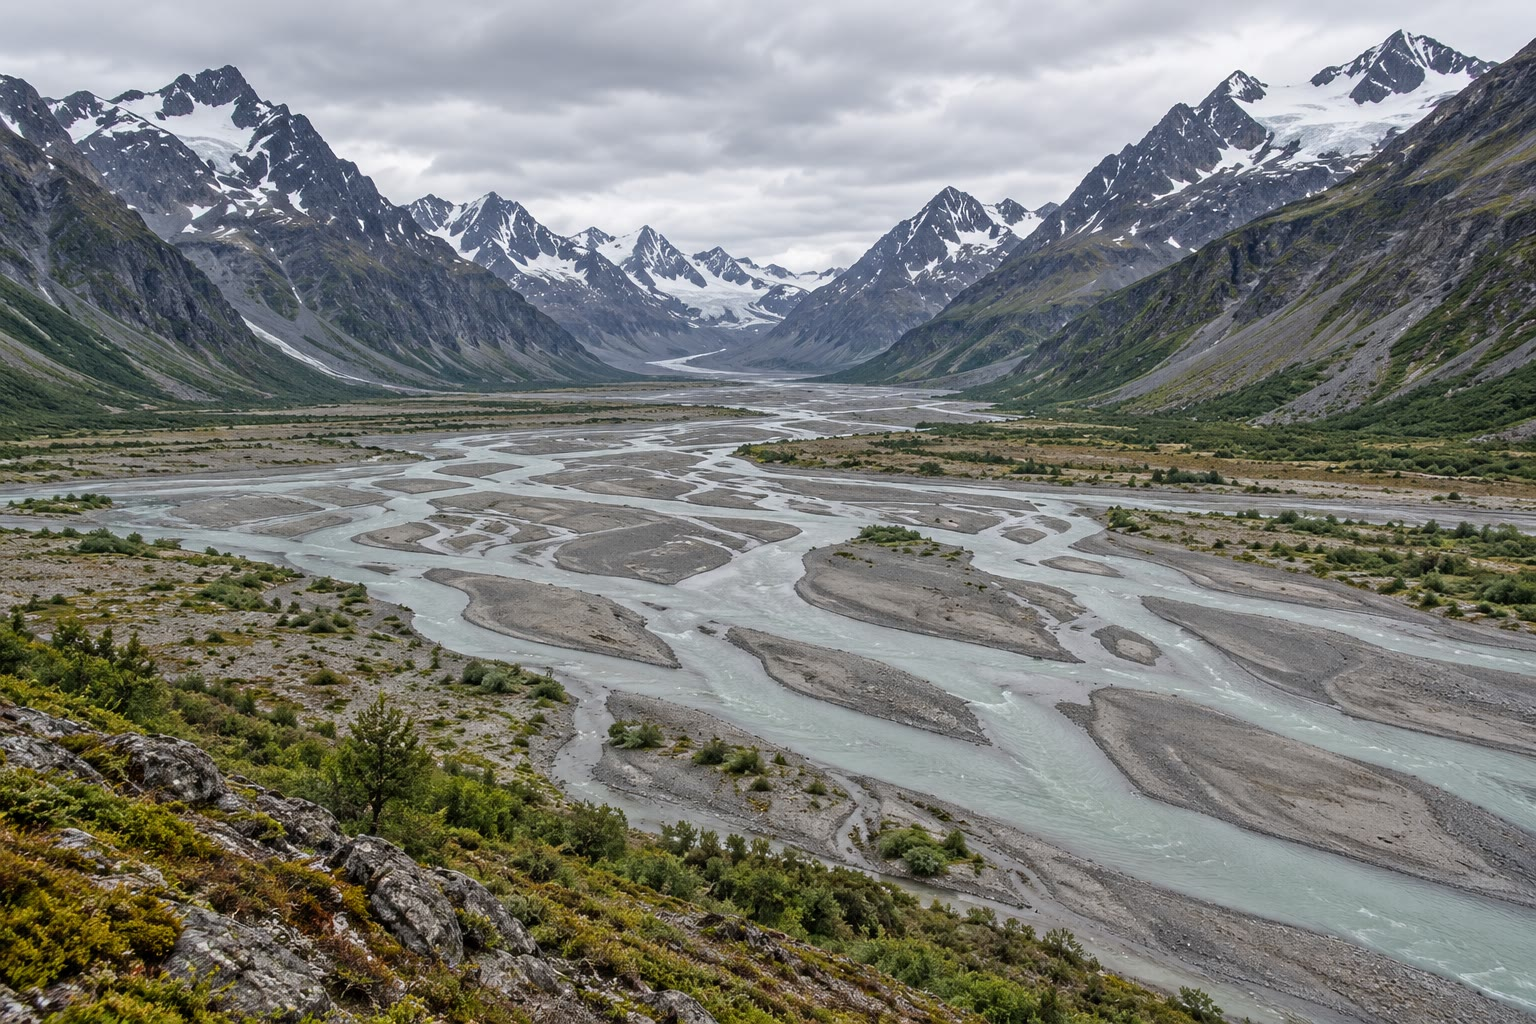
\includegraphics[width=0.66\linewidth]{images/book2/ai/g12-braided-river.jpg}

{\small نهر مضفور في وادٍ جبلي جليدي: قنوات ضحلة تتفرع
ثم تلتقي بين حواجز من الحصى لا يحركها الماء إلا في الفيضانات.
رسم توضيحي مولَّد بالذكاء الاصطناعي.}
\end{omfigure}

قياس ما يحمله النهر طريقة ثانية لإيجاد \omterm{def:g12:destruction-of-mountains:denudation}{معدل التجريد}.

\begin{method}[ميزانية التعرية]\label{met:g12:destruction-of-mountains:budget}
\begin{enumerate}
  \item خذ كتلة الرسوبيات التي يحملها النهر في سنة، وأضف إليها
        \omterm{def:g12:destruction-of-mountains:load}{الحمولة الذائبة} (إن لم تُعرف إلا الحمولة الصلبة، فاقسمها على
        $0.85$).
  \item اقسم على كثافة الصخر، نحو \qty{2830}{kg/m^3} \omterm{def:g12:continental-crust:continental-crust}{للقشرة
        القارية}، لتحصل على حجم الصخر المُزال كل سنة.
  \item اقسم على مساحة \omterm{def:g10:drainage-basins:drainage-basin}{حوض التصريف}: فهذا هو السمك
        المُزال كل سنة.
  \item اضرب في $10^6$ لتعبّر عنه بالأمتار في كل مليون سنة.
\end{enumerate}
\end{method}
% ledger: earle:loads, cm95:crust

\begin{example}[المسيسيبي]\label{ex:g12:destruction-of-mountains:mississippi}
قبل عام 1900، كانت منظومة نهرَي ميزوري--المسيسيبي تحمل نحو 400
مليون طن من الرسوبيات في السنة إلى البحر، من حوض مساحته نحو
\qty{2980000}{km^2}. ومع \omterm{def:g12:destruction-of-mountains:load}{الحمولة الذائبة}، $400/0.85 \approx 471$ مليون
طن، أي $\num{4.71e11}/2830 \approx \qty{1.66e8}{m^3}$ من الصخر في السنة.
وإذا وُزّع ذلك على $\qty{2.98e12}{m^2}$، كان طبقة سمكها
\[
  \frac{\num{1.66e8}}{\num{2.98e12}} \approx \qty{5.6e-5}{m}
  \text{ في السنة، أي نحو } \qty{56}{m/Myr}.
\]
وبين 1987 و2006 لم يحمل النهر إلا 145 مليون طن في السنة، وهذا
يعطي نحو \qty{20}{m/Myr}: فالسدود التي بُنيت على نهر ميزوري في خمسينيات القرن العشرين تحبس
نحو 100 إلى 150 مليون طن في السنة، وتحجز منشآت أخرى أكثر من ذلك.
\end{example}
% ledger: mm10:mississippi, kammerer:mississippi, earle:loads, cm95:crust
% values: miss_before_1900_m_per_myr 55.8, miss_1987_2006_m_per_myr 20.2 (relief_decay.py)

ويمكن إعداد الميزانية نفسها للعالم كله. فقبل أن يغيّر الناس
الأنهار، كانت تحمل نحو 15.5 مليار طن من الرسوبيات الصلبة في السنة إلى
السواحل؛ ومع \omterm{def:g12:destruction-of-mountains:load}{الحمولة الذائبة}، يساوي ذلك نحو \qty{6.4}{km^3} من الصخر في
السنة، تؤخذ من \qty{1.48e8}{km^2} هي مساحة القارات: أي متوسط \omterm{def:g12:destruction-of-mountains:denudation}{معدل تجريد}
يبلغ نحو \qty{43}{m/Myr}، وهو قريب من وسيط قياسات
البيريليوم-10. وقد غيّر الناس منذ ذلك الحين الطرفين كليهما: فتعرية التربة
زادت ما تلتقطه الأنهار بنحو 2.3 مليار طن في السنة، لكن أكثر
من 100 مليار طن من الرسوبيات تستقر الآن خلف السدود.
% ledger: syvitski:modern-flux (Book 1 row, prehuman 15.5 Gt/yr with bed load), sy05:humans, data:etopo1 (land fraction 0.290, grade-11 hypsometry), cm95:crust
% values: world_volume_km3_per_yr 6.44, land_area_km2 1.48e8, world_m_per_myr 43.5 (relief_decay.py)

\section{من الرسوبيات إلى الصخر}

تُرسَّب حمولة الأنهار حيث يتباطأ التيار: في الأودية والبحيرات،
وعلى الدلتاوات، وقبل كل شيء في \omterm{def:g11:fossil-fuel-geology:basin}{الأحواض الرسوبية} للحواف
القارية. وطبقة بعد طبقة، تُدفن الرسوبيات،
وتتحول ببطء إلى صخر.

\begin{definition}[الصخر الفتاتي؛ التصخّر]\label{def:g12:destruction-of-mountains:diagenesis}
\emph{الصخر الفتاتي}\index{صخر فتاتي} (أو الصخر الحطامي) صخر
رسوبي مكوّن من قطع، هي الفتات، من صخور ومعادن أقدم.
و\emph{التصخّر}\index{تصخّر} مجموعة التغيرات التي تحوّل رسوبيات
مدفونة إلى صخر عند درجة حرارة منخفضة: \emph{التراص}، إذ يعصر ثقل
الطبقات التي فوقها الماء والهواء فيطردهما، ثم \emph{الالتحام}، إذ
تلصق الحبيبات بعضها ببعض معادن تتبلور من الماء الذي في المسام (الكالسيت،
والكوارتز، والهيماتيت، \omterm{def:g10:soil-formation:clay}{والمعادن الطينية}).
\end{definition}
% ledger: earle:clastic

تُسمّى الصخور الفتاتية بحسب حجم فتاتها:
\begin{itemize}
  \item \textbf{الرصيص} مكوّن من فتات مستدير أكبر من
        \qty{2}{mm}، و\textbf{البريشيا} من فتات زاوي؛
  \item \textbf{الحجر الرملي} مكوّن من الرمل، أي حبيبات بين \qty{2}{mm}
        و\qty{0.063}{mm}، وهي في الغالب من الكوارتز، المعدن الأشد
        مقاومة للتجوية؛
  \item \textbf{الصخر الطيني} يحوي \qty{75}{\percent} على الأقل من الغرين والطين؛
        وهو سجيل إذا انفلق إلى طبقات رقيقة.
\end{itemize}
% ledger: earle:clastic

\begin{omfigure}
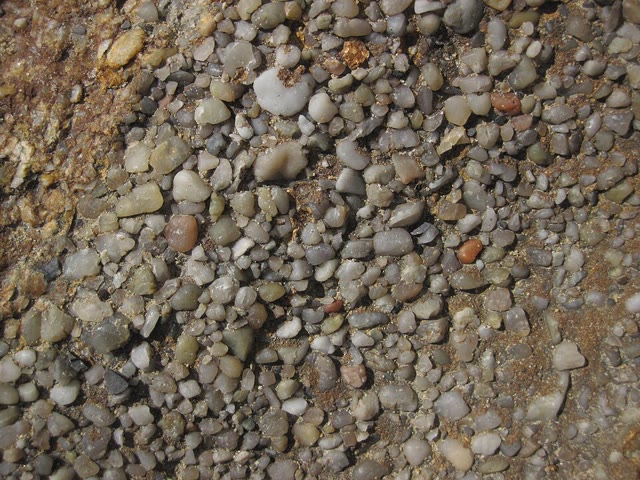
\includegraphics[width=0.5\linewidth]{images/book2/g12-stjohn-conglomerate.jpg}

{\small رصيص من حصى الكوارتز من أوهايو، من العصر الكربوني:
حصى مستديرة من الكوارتز، يلحمها رمل أدق. الصورة: جيمس
سانت~جون (CC~BY~2.0).}
\end{omfigure}
% ledger: photo:g12-conglomerate, ics:base.Carboniferous, ics:base.Permian (Lower Pennsylvanian lies in the Carboniferous)

الفتات يسجّل الرحلة. فالحصى المستديرة تدحرجت مسافة طويلة في
نهر أو على شاطئ؛ أما الزاوية فلم تكد تنتقل. والحجر الرملي المكوّن
من الكوارتز وحده تقريبًا يأتي من صخر تعرّض للتجوية زمنًا طويلًا،
حتى تحولت المعادن الأخرى إلى طين.
% ledger: earle:clastic (rounded/angular, most sand grains quartz, the most resistant mineral)

\section{الجذر يرتفع}

لو كانت التعرية تزيل الصخر من أعلى السلسلة فحسب، لزالت سلسلة ارتفاعها \qty{2}{km}،
تُبرى بمعدل \qty{200}{m/Myr}، في عشرة ملايين سنة.
لكن السلسلة تطفو على الوشاح. فكلما أُزيل الصخر من أعلاها،
خفّ العمود، فارتفع.

\begin{definition}[الارتداد الأيزوستاتي]\label{def:g12:destruction-of-mountains:rebound}
\emph{الارتداد الأيزوستاتي}\index{ارتداد أيزوستاتي} هو ارتفاع منطقة من
\omterm{def:g11:lithosphere-asthenosphere:lithosphere}{الغلاف الصخري} حين يُزال عنها حمل --- صخر تبريه التعرية،
أو غطاء جليدي يذوب --- إلى أن يعود \omterm{def:g11:lithosphere-asthenosphere:isostasy}{التوازن الأيزوستاتي}.
\end{definition}
% ledger: sella07:gia (rebound after ice unloading)

\begin{proposition}[التعرية والارتداد]\label{prop:g12:destruction-of-mountains:rebound}
في نموذج إيري، حين تزيل التعرية سمكًا $e$ من قشرة كثافتها
$\rho_c$ من منطقة في \omterm{def:g11:lithosphere-asthenosphere:isostasy}{توازن أيزوستاتي} على وشاح كثافته $\rho_m$، فإن
السطح لا ينخفض إلا بمقدار
\[
  \Delta h = e\left(1 - \frac{\rho_c}{\rho_m}\right),
\]
بينما ترتفع قاعدة القشرة بمقدار $e\,\rho_c/\rho_m$.
\end{proposition}

\begin{proof}
إزالة $e$ من الأعلى تجعل القشرة أرق بمقدار $e$. وبحسب نموذج إيري،
تقف القشرة الأرق بمقدار $e$ أخفض بمقدار $e\,(\rho_m - \rho_c)/\rho_m = e(1 -
\rho_c/\rho_m)$. فقد انخفض أعلى القشرة بهذا المقدار، ونقص
سمكها بمقدار $e$، إذن ارتفعت قاعدتها بمقدار $e - e(1 -
\rho_c/\rho_m) = e\,\rho_c/\rho_m$.
\end{proof}
مع $\rho_c = \qty{2830}{kg/m^3}$ و$\rho_m = \qty{3380}{kg/m^3}$، يكون $1 -
\rho_c/\rho_m \approx 0.163$. فإزالة \qty{1}{km} من الصخر لا تخفض
السطح إلا بنحو \qty{163}{m}: أما \qty{837}{m} الباقية فيعوّضها
ارتفاع العمود كله.
ولخفض سلسلة بمقدار \qty{2000}{m}، يجب أن تزيل التعرية
نحو $2000/0.163 \approx \qty{12300}{m}$ من الصخر. فالصخور التي كانت على عمق
يزيد على \qty{12}{km}، من صخور متحولة وغرانيتات تكوّنت في أعماق
السلسلة، تبلغ السطح: ولهذا تكشف الأحزمة الجبلية القديمة المبريّة
عن الشيست والنيس والغرانيت على مساحات شاسعة.
% ledger: cm95:crust, data:prem (rho 3.38 below the Moho)
% values: rebound_fraction 0.16272, lowering_per_km_m 162.7, root_rise_per_km_m 837.3, eroded_for_2000m_km 12.29 (relief_decay.py)

\begin{omfigure}
\begin{tikzpicture}[x=1cm, y=1cm, font=\scriptsize]
  % three columns: before, after erosion without rebound, after rebound
  \foreach \i/\top/\base/\lab in {0/3.0/-3.2/{سلسلة في توازن أيزوستاتي}, 1/2.0/-3.2/{\foreignlanguage{arabic}{التعرية تزيل $e$}}, 2/2.84/-2.36/{العمود يرتفع}} {
    \begin{scope}[xshift=\i*4.6cm]
      \fill[omLithPeridotite!45] (0,-3.6) rectangle (3.4,-0.6);
      \fill[omLithGranite!55, draw=black!60] (0.5,\base) -- (0.5,0) -- (1.0,\top) -- (2.4,\top) -- (2.9,0) -- (2.9,\base) -- cycle;
      \fill[omLithGranite!55, draw=black!60] (0,0) rectangle (0.5,-0.6);
      \fill[omLithGranite!55, draw=black!60] (2.9,0) rectangle (3.4,-0.6);
      \draw[black!40, densely dashed] (-0.1,0) -- (3.5,0);
      \node[anchor=north, align=center, text width=3.4cm] at (1.7,-3.75) {\lab};
    \end{scope}
  }
  % eroded slab, middle panel
  \draw[omThm, densely dashed] (4.6+1.0,3.0) -- (4.6+2.4,3.0);
  \draw[omThm, |-|] (4.6+2.65,3.0) -- node[right] {$e$} (4.6+2.65,2.0);
  % right panel: the old top and base
  \draw[omThm, densely dashed] (9.2+1.0,3.0) -- (9.2+2.4,3.0);
  \draw[omThm, densely dashed] (9.2+0.5,-3.2) -- (9.2+2.9,-3.2);
  \draw[-{Stealth}, omDef, line width=0.9pt] (9.2+1.7,-3.15) -- (9.2+1.7,-2.45);
  \node[omDef, anchor=west] at (9.2+3.0,-2.8) {الجذر يرتفع};
  \node[anchor=west] at (9.2+3.0,2.95) {ينخفض السطح};
  \node[anchor=west] at (9.2+3.0,2.55) {\foreignlanguage{arabic}{بمقدار $0.16\,e$ فقط}};
  \draw[black!60, |-|] (9.2+2.65,3.0) -- (9.2+2.65,2.84);
  % labels
  \node[anchor=west] at (3.45,-2.1) {الوشاح};
  \node at (1.7,-1.5) {القشرة};
\end{tikzpicture}

{\small التعرية \omterm{def:g12:destruction-of-mountains:rebound}{والارتداد الأيزوستاتي} (رسم تخطيطي، الارتفاعات ليست بمقياس رسم). في اليسار:
سلسلة في \omterm{def:g11:lithosphere-asthenosphere:isostasy}{توازن أيزوستاتي}، \omterm{def:g12:continental-crust:root}{بجذرها}. في الوسط: التعرية تزيل سمكًا $e$
من الأعلى. في اليمين: العمود الأخف يرتفع إلى أن يعود \omterm{def:g11:lithosphere-asthenosphere:isostasy}{التوازن الأيزوستاتي}؛ فلا
ينتهي السطح إلا أخفض بمقدار $0.163\,e$ مما كان في البداية، ويكون \omterm{def:g12:continental-crust:root}{الجذر} قد ارتفع
بمقدار $0.837\,e$.}
\end{omfigure}

ويمكن رصد هذا الارتداد نفسه اليوم حيث زال حمل بسرعة. فالغطاء
الجليدي الذي غطى معظم كندا في الذروة الجليدية الأخيرة كان
أسمك ما يكون حول خليج هدسون. وقد ذاب ذلك الجليد، ولا تزال الأرض هناك
ترتفع: بنحو \qty{10}{mm} في السنة، كما تقيسها أجهزة تحديد المواقع بالأقمار الصناعية، أي
\qty{10000}{m/Myr}، وهذا نحو خمسين ضعف متوسط \omterm{def:g12:destruction-of-mountains:denudation}{معدل تجريد} أحواض
\omterm{def:g10:drainage-basins:discharge}{التصريف}. وأبعد جنوبًا،
وراء البحيرات العظمى، تهبط الأرض بمقدار 1 إلى \qty{2}{mm} في السنة.
% ledger: sella07:gia, pb11:rates

\section{كم تدوم السلسلة الجبلية؟}

كلما اشتد انحدار الحوض، أسرعت تعريته؛ وقد وُجد أن \omterm{def:g12:destruction-of-mountains:denudation}{معدل التجريد}
في الأحواض الكبيرة يتناسب مع متوسط تضاريسها. فلنأخذ
أبسط نموذج يعبّر عن ذلك.

\begin{proposition}[التناقص الأسي للسلسلة الجبلية]\label{prop:g12:destruction-of-mountains:decay}
ليكن $h(t)$ متوسط ارتفاع سلسلة فوق السهول المحيطة بها. إذا كان
\omterm{def:g12:destruction-of-mountains:denudation}{معدل التجريد} $E = k\,h$، حيث $k$ ثابت، وكان \omterm{def:g11:lithosphere-asthenosphere:isostasy}{التوازن الأيزوستاتي}
يُستعاد في كل لحظة، فإن
\[
  h(t) = h_0\, e^{-f k t}, \qquad f = 1 - \frac{\rho_c}{\rho_m},
\]
حيث $h_0$ الارتفاع عند $t = 0$. فالارتفاع ينقسم على $e$
كل $\tau = 1/(fk)$، وعلى اثنين كل $\tau \ln 2$.
\end{proposition}

\begin{proof}
في زمن قصير $\mathrm{d}t$، تزيل التعرية سمكًا $E\,\mathrm{d}t
= k h\,\mathrm{d}t$، وبحسب القضية السابقة ينخفض السطح
بمقدار $f k h\,\mathrm{d}t$. إذن $h' = -fk\,h$، وحلول هذه
المعادلة هي $h(t) = h_0\,e^{-fkt}$. وعند $t = \tau$، يكون $h = h_0/e$؛ ويكون $h = h_0/2$
عندما $fkt = \ln 2$.
\end{proof}

تعطي القياسات على الأحواض الكبيرة قيمة $k$: فلو لم يكن هناك رفع على الإطلاق، لانخفضت
تضاريسها إلى العُشر في نحو 11 مليون سنة. إذن $e^{-11k} = 0.1$، و$k =
\ln 10/11 \approx 0.209$ في كل مليون سنة. ودون ارتداد ($f = 1$)، يكون
الثابت الزمني $1/k \approx 4.8$ مليون سنة. ومع الارتداد، $f
\approx 0.163$
و\[
  \tau = \frac{1}{0.163 \times 0.209} \approx 29 \text{ مليون سنة},
\]
وينتصف متوسط الارتفاع كل $29 \ln 2 \approx 20$ مليون سنة:
فالارتداد يجعل السلسلة تدوم أطول بنحو ست مرات.
% ledger: ahnert70:decay, cm95:crust, data:prem
% values: k_per_myr 0.20933, tau_none_myr 4.777, tau_rebound_myr 29.36, half_rebound_myr 20.35, half_none_myr 3.31 (relief_decay.py)

\begin{omfigure}
\begin{tikzpicture}
\begin{axis}[omrecord, width=0.7\linewidth, height=5.4cm, xmin=0, xmax=100, ymin=0, ymax=2100,
  xlabel={\foreignlanguage{arabic}{الزمن بملايين السنين}}, ylabel={\foreignlanguage{arabic}{متوسط الارتفاع \babelsublr{(\unit{m})}}},
  xtick={0,20,...,100}, ytick={0,500,...,2000}]
% computed in figdata/grade-12/relief_decay.py; ledger: ahnert70:decay, cm95:crust, data:prem
\addplot[omProp, line width=1.1pt, densely dashed] table[x=t_Myr, y=h_none] {figdata/out/grade-12-relief_decay-curve.dat};
\addplot[omDef, line width=1.1pt] table[x=t_Myr, y=h_rebound] {figdata/out/grade-12-relief_decay-curve.dat};
\draw[black!45, densely dotted] (axis cs:20.35,0) -- (axis cs:20.35,1000) -- (axis cs:0,1000);
\draw[omProp, line width=0.4pt] (axis cs:9,304) -- (axis cs:33,215);
\coordinate (none) at (axis cs:33.5,215);
\coordinate (reb) at (axis cs:45,780);
\end{axis}
\node[font=\scriptsize, text=omProp, anchor=west] at (none) {دون ارتداد};
\node[font=\scriptsize, text=omDef, anchor=south west] at (reb) {مع الارتداد};
\end{tikzpicture}

{\small متوسط ارتفاع سلسلة علوها \qty{2000}{m}، تُبرى بمعدل
يتناسب مع ارتفاعها، مع \omterm{def:g12:destruction-of-mountains:rebound}{الارتداد الأيزوستاتي} ودونه؛ ومع
الارتداد، يبقى نصف الارتفاع بعد 20 مليون سنة (الخط المنقط). ثابت
المعدل من أنيرت (1970)؛ وكثافتا القشرة والوشاح الذي تحت
\omterm{def:g11:seismic-structure:moho}{الموهو}.}
\end{omfigure}

جبال الأبالاش تختبر هذه الصورة. فقد انتهى اصطدامها في البرمي،
قبل أكثر من 250 مليون سنة. وهذا أكثر من اثني عشر ضعف الزمن الذي
يستغرقه النموذج لينصّف الارتفاع: $2000 \times e^{-250/29} \approx
\qty{0.4}{m}$. ومع ذلك لا يزال جبل ميتشل يرتفع \qty{2037}{m} فوق البحر.
فالنموذج وحده لا يفسر التضاريس الحالية: لا بد أن المنطقة
رُفعت من جديد منذ ذلك الحين، أو تعرّت أبطأ مما يفترض النموذج.
% ledger: usgs:alleghanian, usgs:alleghanian-age, ics:base.Triassic, ncparks:mitchell, ahnert70:decay
% values: h_after_250myr_rebound_m 0.40 (relief_decay.py)

فالجبال إذن يُعاد تدويرها. فالصخر المبريّ من سلسلة ينتهي إلى \omterm{def:g11:fossil-fuel-geology:basin}{أحواض
رسوبية}، فيصير فيها صخرًا فتاتيًا؛ ويُدفن بعض ذلك الصخر عميقًا
بما يكفي ليتحول أو حتى لينصهر، ويُحمل بعضه إلى الوشاح
في \omterm{def:g11:subduction-zones:subduction}{نطاق اندساس} (\cref{ch:g12:subduction-magmatism})، ويُطوى بعضه
من جديد في سلسلة جديدة حين تتصادم قارتان.
% ledger: ss09:balance (sediment subducted), earle:collision (sediments of both margins in the mountains)

\begin{omfigure}
\begin{tikzpicture}
\begin{axis}[omsection, x=1.25cm, y=0.003125cm, xmin=0, xmax=9.49, ymin=-700, ymax=650,
  xlabel={\foreignlanguage{arabic}{المسافة من A \babelsublr{(\unit{km})}}}, ylabel={\foreignlanguage{arabic}{الارتفاع \babelsublr{(\unit{m})}}},
  ytick={-600,-300,0,300,600}, tick label style={font=\scriptsize}, unbounded coords=jump]
% shared region tables (figdata/shared/region.py); unconformity from figdata/grade-12/relief_decay.py; ledger: region:name
\addplot[fill=black!8, draw=black!50, line width=0.3pt, even odd rule] table {figdata/out/shared-region-section-unit-schist.dat};
\addplot[fill=icsTriassic!20, draw=black!50, line width=0.3pt, even odd rule] table {figdata/out/shared-region-section-unit-sandstone.dat};
\addplot[fill=icsJurassic!25, draw=black!50, line width=0.3pt, even odd rule] table {figdata/out/shared-region-section-unit-limestone.dat};
\addplot[fill=icsJurassic!8, draw=black!50, line width=0.3pt, even odd rule] table {figdata/out/shared-region-section-unit-shale.dat};
\addplot[fill=icsCretaceous!20, draw=black!50, line width=0.3pt, even odd rule] table {figdata/out/shared-region-section-unit-chalk.dat};
\addplot[fill=omLithAlluv, draw=black!50, line width=0.3pt, even odd rule] table {figdata/out/shared-region-section-unit-alluvium.dat};
\addplot[black, line width=0.7pt] table {figdata/out/shared-region-section-ground.dat};
\addplot[omThm, line width=1.4pt] table[x=s_km, y=z_m] {figdata/out/grade-12-relief_decay-unconformity.dat};
\addplot[fault] table {figdata/out/shared-region-section-fault.dat};
\node[anchor=south east, font=\small\bfseries] at (axis cs:0,650) {A};
\node[anchor=south west, font=\small\bfseries] at (axis cs:9.49,650) {B};
\node[font=\scriptsize, fill=white, inner sep=1pt] at (axis cs:1.2,-520) {\foreignlanguage{arabic}{شيست، نحو 480 مليون سنة}};
\coordinate (unc) at (axis cs:1.6,-300);
\end{axis}
\node[font=\scriptsize, text=omThm, anchor=west, fill=white, inner sep=1pt] at ([xshift=4pt]unc) {سطح عدم التوافق};
\end{tikzpicture}

\smallskip
{\small\tikz\fill[black!8, draw=black!50] (0,0) rectangle (0.35,0.22);~شيست \quad
\tikz\fill[icsTriassic!20, draw=black!50] (0,0) rectangle (0.35,0.22);~حجر رملي ترياسي \quad
\tikz\fill[icsJurassic!25, draw=black!50] (0,0) rectangle (0.35,0.22);~حجر جيري \quad
\tikz\fill[icsJurassic!8, draw=black!50] (0,0) rectangle (0.35,0.22);~سجيل \quad
\tikz\fill[icsCretaceous!20, draw=black!50] (0,0) rectangle (0.35,0.22);~طباشير \quad
\omve{2.5}}

{\small المقطع A--B عبر تلال فاردن، وسطح عدم التوافق بالأحمر:
القاعدة المستوية التي ترسب عليها الحجر الرملي الترياسي فوق قاعدة
الشيست، ثم طُويت وتصدّعت لاحقًا. البيانات: نموذج السلسلة للمنطقة.}
\end{omfigure}
% values: unconformity sampled from region.contact_elevation('sandstone'); varden_gap_myr 58.1 (relief_decay.py)

تحفظ تلال فاردن سجل دورة كهذه. فقاعدتها شيست
تحوّل قبل نحو 480 مليون سنة، اقتحمه غرانيت قبل
نحو 310 ملايين سنة --- وكلاهما تكوّن على عمق كيلومترات تحت سطح
حزام جبلي قديم. ومع ذلك فالحجر الرملي الترياسي، الذي ترسب منذ نحو 252
مليون سنة، يستقر عليهما مباشرة، عبر سطح مستوٍ: هو سطح
عدم التوافق. ففي أقل من 60 مليون سنة، كانت تلك السلسلة القديمة قد بُريت
حتى صارت سهلًا وبلغت صخورها العميقة السطح. ثم امتد البحر
فوق السهل ودفنه.
% ledger: region:name (model: schist 480 Ma, granite 310 Ma, erosion, unconformity, Triassic cover), ics:base.Triassic
% values: varden_gap_myr 58.1 (relief_decay.py)

\section{تمارين}

\begin{exercise}[$\star$]\label{exo:g12:destruction-of-mountains:1}
أعطِ المصطلح: (أ) متوسط سمك الصخر الذي يُزال من منطقة في وحدة
الزمن؛ (ب) الحبيبات التي يدحرجها النهر ويقفز بها على طول قاعه؛ (ج)
الأيونات التي يحملها النهر في محلول؛ (د) التغيرات التي تحوّل رسوبيات مدفونة
إلى صخر؛ (ه) ارتفاع \omterm{def:g11:lithosphere-asthenosphere:lithosphere}{الغلاف الصخري} حين يُزال عنه حمل.
\end{exercise}

\begin{exercise}[$\star$]\label{exo:g12:destruction-of-mountains:2}
سمِّ \omterm{def:g12:destruction-of-mountains:diagenesis}{الصخر الفتاتي}: (1) حصى مستديرة قطرها \qtyrange{5}{20}{mm}
ملتحمة معًا؛ (2) حبيبات كوارتز قطرها \qty{0.3}{mm}؛ (3) صخر
\qty{90}{\percent} منه غرين وطين وينفلق إلى صفائح رقيقة؛ (4) قطع
زاوية طولها \qty{3}{cm}.
\end{exercise}

\begin{exercise}[$\star$]\label{exo:g12:destruction-of-mountains:3}
حوّل إلى ملّيمترات في السنة: (1) \qty{54}{m/Myr}؛ (2) \qty{218}{m/Myr}؛
(3) وحوّل ارتفاع \qty{10}{mm} في السنة قرب خليج هدسون إلى \unit{m/Myr}.
\end{exercise}

\begin{exercise}[$\star$]\label{exo:g12:destruction-of-mountains:4}
يحمل نهر 60 مليون طن من الرسوبيات الصلبة في السنة. قدّر
حمولته الذائبة، علمًا بأن \omterm{def:g12:destruction-of-mountains:load}{الحمولة الذائبة} تبلغ في المتوسط
\qty{15}{\percent} من الكتلة الكلية المحمولة.
\end{exercise}

\begin{exercise}[$\star$]\label{exo:g12:destruction-of-mountains:5}
رتّب، من السطح نحو الأسفل، ما يحدث لحبيبة كوارتز
من غرانيت: الترسيب في حوض، وتجوية الغرانيت، والدفن تحت
طبقات أحدث، والنقل بنهر، والالتحام.
\end{exercise}

\begin{exercise}[$\star\star$]\label{exo:g12:destruction-of-mountains:6}
يتباطأ تيار من \qty{30}{cm/s} إلى \qty{5}{cm/s}. مستعينًا بقيم
الفصل، قل ما يحدث لحبيبة رمل قطرها \qty{1}{mm} مستقرة على
القاع، ولحبيبة غرين قطرها \qty{0.01}{mm} عالقة أصلًا، عند
كل سرعة.
\end{exercise}

\begin{exercise}[$\star\star$]\label{exo:g12:destruction-of-mountains:7}
حوض مساحته \qty{50000}{km^2} يرسل 4 ملايين طن من الرسوبيات الصلبة في السنة
إلى البحر. أعدّ ميزانية تعريته، شاملة \omterm{def:g12:destruction-of-mountains:load}{الحمولة الذائبة}، مع $\rho =
\qty{2830}{kg/m^3}$. وقارنها بوسيط معدلات الأحواض المقيسة بالبيريليوم-10.
\end{exercise}

\begin{exercise}[$\star\star$]\label{exo:g12:destruction-of-mountains:8}
(1) احسب $1 - \rho_c/\rho_m$ حين $\rho_c = \qty{2700}{kg/m^3}$
و$\rho_m = \qty{3300}{kg/m^3}$. (2) بكم ينخفض السطح حين
يُعرّى \qty{1}{km} من الصخر؟ (3) قارن بقيمة الفصل.
\end{exercise}

\begin{exercise}[$\star\star$]\label{exo:g12:destruction-of-mountains:9}
تبلور غرانيت على عمق نحو \qty{8}{km} تحت سلسلة جبلية. (1) ما
سمك الصخر الذي يجب أن تزيله التعرية لتبلغ به السطح؟ (2) بكم
ينخفض متوسط السطح في أثناء ذلك؟ (3) بمعدل \qty{200}{m/Myr}،
كم يستغرق ذلك؟
\end{exercise}

\begin{exercise}[$\star\star$]\label{exo:g12:destruction-of-mountains:10}
يبلغ متوسط ارتفاع القارات نحو \qty{794}{m}. (1) بمعدل
\qty{43}{m/Myr}، كم تستغرق التعرية لتزيل طبقة بهذا السمك؟
(2) وكم تستغرق إذا أُخذ \omterm{def:g12:destruction-of-mountains:rebound}{الارتداد الأيزوستاتي} في الحسبان وبقي المعدل
على حاله؟ (3) لماذا تظل القارات مع ذلك فوق مستوى البحر
بعد 4 مليارات سنة؟
\end{exercise}

\begin{exercise}[$\star\star$]\label{exo:g12:destruction-of-mountains:11}
تستقر أكثر من 100 مليار طن من الرسوبيات خلف سدود بُني معظمها في
الخمسين سنة الأخيرة. (1) ما حجم الصخر الذي يمثله ذلك، بكثافة
\qty{2830}{kg/m^3}؟ (2) كم سنة من الحمولة الصلبة العالمية قبل تدخل الإنسان،
15.5 مليار طن في السنة، يمثل ذلك؟
\end{exercise}

\begin{exercise}[$\star\star\star$]\label{exo:g12:destruction-of-mountains:12}
بيّن أن \omterm{def:g12:destruction-of-mountains:denudation}{معدل تجريد} سلسلة جبلية، في نموذج الفصل، هو
$E(t) = k h_0 e^{-fkt}$. واحسب السمك الكلي للصخر المُزال بينما
ينخفض متوسط الارتفاع من $h_0$ إلى 0، وفسّر النتيجة بقضية
الارتداد.
\end{exercise}

\begin{exercise}[$\star\star\star$]\label{exo:g12:destruction-of-mountains:13}
قرب خليج هدسون ترتفع الأرض بمقدار \qty{10}{mm} في السنة. (1) لو بقي ذلك المعدل
على حاله، فكم ترتفع في 1000 سنة؟ (2) هذا الارتفاع
ارتداد بعد ذوبان غطاء جليدي. خذ جليدًا كثافته
\qty{900}{kg/m^3} ووشاحًا كثافته \qty{3380}{kg/m^3}: كم ترتفع
الأرض في المجموع، في نموذج إيري، بعد ذوبان \qty{2}{km} من الجليد؟
(3) لماذا ينبغي أن يتباطأ المعدل مع الزمن؟
\end{exercise}
% ledger: sella07:gia, usgs:ice-density (ice about 90 % as dense as water), data:prem

\begin{exercise}[$\star\star\star$]\label{exo:g12:destruction-of-mountains:14}
كان المسيسيبي يحمل 400 مليون طن من الرسوبيات الصلبة في السنة قبل
عام 1900، و145 مليون طن في السنة في الفترة 1987--2006. (1) احسب
\omterm{def:g12:destruction-of-mountains:denudation}{معدل تجريد} حوضه البالغة مساحته \qty{2980000}{km^2} في الفترتين، مع
\omterm{def:g12:destruction-of-mountains:load}{الحمولة الذائبة}. (2) أي القيمتين يقيس التعرية الطبيعية
للحوض قياسًا أفضل؟ (3) تحبس السدود من 100 إلى 150 مليون طن في السنة: فهل يفسر ذلك
النقص كله؟
\end{exercise}

\begin{exercise}[$\star\star\star$]\label{exo:g12:destruction-of-mountains:15}
في تلال فاردن، يقع غرانيت اقتحم الصخور قبل نحو 310 ملايين سنة
تحت حجر رملي ترياسي، ترسب منذ نحو 252 مليون سنة.
افترض أن الغرانيت تبلور على عمق \qty{6}{km}. (1) ما سمك الصخر
الذي أُزيل فوقه، على الأقل؟ (2) ما متوسط \omterm{def:g12:destruction-of-mountains:denudation}{معدل التجريد} الذي يتطلبه
ذلك، على الأقل؟ (3) قارن بالمعدلات المقيسة للأحواض.
\end{exercise}

\begin{problem}[{مسألة نهاية الأسبوع --- كم يستغرق تسوية سلسلة جبلية؟}]
\label{pb:g12:destruction-of-mountains:1}
% ledger: pb11:rates, ahnert70:decay, cm95:crust, data:prem, usgs:alleghanian, usgs:alleghanian-age, ics:base.Triassic, ncparks:mitchell, photo:g12-appalachians
% values (relief_decay.py): k 0.20933/Myr, E0 418.7 m/Myr, f 0.16272, tau 4.777 / 29.36 Myr, half-lives 3.31 / 20.35 Myr
لسلسلة فتية متوسط ارتفاع يبلغ \qty{2000}{m} فوق السهول المحيطة
بها. وأنهارها تبريها بمعدل يتناسب مع ارتفاعها، $E = kh$،
حيث $k = 0.209$ في كل مليون سنة. وكثافة القشرة
\qty{2830}{kg/m^3}، وكثافة الوشاح الذي تحتها \qty{3380}{kg/m^3}.

\medskip
\noindent\textbf{الجزء الأول --- معدل التعرية.}
\begin{enumerate}
  \item احسب \omterm{def:g12:destruction-of-mountains:denudation}{معدل تجريد} السلسلة اليوم، بوحدة \unit{m/Myr}.
  \item عبّر عنه بالملّيمترات في السنة.
  \item قارنه بمتوسط المعدلات المقيسة في الأحواض النشطة زلزاليًا
        (\qty{367}{m/Myr}) وفي الأحواض الهادئة (\qty{182}{m/Myr}).
  \item ما خاصية الحوض التي تتنبأ بمعدل تعريته أفضل من غيرها؟
  \item كم طنًا من الصخر يغادر كل كيلومتر مربع من السلسلة
        كل سنة؟
\end{enumerate}

\medskip
\noindent\textbf{الجزء الثاني --- دون ارتداد.}
\begin{enumerate}[resume]
  \item لو بقي المعدل على قيمته الحالية، فكم يستغرق
        إزالة \qty{2000}{m} من الصخر؟
  \item في الواقع ينخفض المعدل كلما انخفضت السلسلة. اكتب المعادلة
        $h' = -kh$ وحلها مع $h(0) = \qty{2000}{m}$.
  \item ما الثابت الزمني $1/k$؟
  \item كم يستغرق الارتفاع لينتصف؟
  \item تحقق من أن عُشر الارتفاع يبقى بعد 11 مليون سنة.
\end{enumerate}

\medskip
\noindent\textbf{الجزء الثالث --- مع الارتداد.}
\begin{enumerate}[resume]
  \item احسب $f = 1 - \rho_c/\rho_m$.
  \item حين يُعرّى \qty{100}{m} من الصخر، بكم ينخفض
        السطح، وبكم يرتفع \omterm{def:g12:continental-crust:root}{الجذر}؟
  \item اكتب المعادلة الجديدة التي يحققها $h$، وحلها.
  \item ما سمك الصخر الذي يجب أن يُعرّى لخفض السلسلة من
        \qty{2000}{m} إلى \qty{200}{m}؟
  \item ما أنواع الصخور التي يجلبها ذلك إلى السطح؟
\end{enumerate}

\medskip
\noindent\textbf{الجزء الرابع --- الثابت الزمني.}
\begin{enumerate}[resume]
  \item احسب الثابت الزمني مع الارتداد.
  \item كم تستغرق السلسلة لتنخفض إلى عُشر ارتفاعها؟
  \item كم يبلغ ارتفاعها بعد 200 مليون سنة؟
  \item انتهى اصطدام الأبالاش قبل أكثر من 250 مليون سنة.
        لو لم تُرفع السلسلة من جديد قط، فكم يكون ارتفاعها بحسب النموذج
        بعد 250 مليون سنة؟ لا يزال جبل ميتشل يرتفع \qty{2037}{m}
        فوق البحر: فماذا يوحي ذلك؟
  \item لخّص: في كم مليون سنة ينتصف متوسط ارتفاع
        السلسلة؟
\end{enumerate}
\end{problem}
